\chapter{Transformations of Symmetry}\label{Chap:Subgroups}

When determining the structure of a material, one should not assume that when a good, or even excellent, fit to the experimental data is found that this indicates that the structural model is correct. 
There may be other models that fit better that have not yet been found. 
Even if it is known that the model offers the best fit to a set of experimental data, it may be that with more precise data, it would be clear that a different model is to be preferred. There is also the problem of ``fitting noise'': Sometimes, in order to improve the fit, refinement will distort a model in ways that are not chemically reasonable. If refinement improves the fit to data by distorting a phenyl group so it is no longer planar and the C-C bond lengths are unequal, that model would be far less plausible, even though it provides a better fit to the data than a chemically reasonable model. 

Perhaps a better question than ``what is the correct model?'' would be ``what is the most accurate structure that is consistent with a set of data?'' since with better data, one may be able to learn more. A key question will be to establish the best symmetry description for the structure. Crystallographers have traditionally been very concerned about missing symmetry. When a structure is refined in too low a space group, the missing symmetry will invariably degrade the quality of the refinement. Historically, the highly respected Caltech crystallographer Richard Marsh\index{Marsh, R.}, who died in 1994, published reports on crystal structures where symmetry had been missed. Invariably, the higher-symmetry structure was preferred, and often removed implausible aspects in chemistry. Dick was a pleasure to be around. I am not the only one who misses him. The process of finding a higher symmetry space group for published work is often referred to as ``Marshing'' in his honor. 

If the space group used for the model is too high, then the structure will be inaccurate because the symmetry will force details of the structure conform to symmetry elements that are not present, for example by requiring elements to lie on or be reflected by a mirror plane that is not actually present. When the symmetry is too high, the model will miss key details in how the structure deviates from that falsely imposed symmetry. 
When it is found that a structure is in too high a space group, there are at least a few of us that call this ``Anti-Marshing''. While data quality limits the ability to determine structures, my personal feeling is that using too high symmetry is actually a bigger problem than missing symmetry. As an example, reporting that a material is centrosymmetric when it is actually acentric will cause some interesting science to be missed. 

\section{Subgroup and Supergroup Relationships}\index{subgroup}\index{supergroup}

When exploring symmetry symmetry choices, it is very valuable to understand that space groups are linked together by the addition or removal of symmetry. Given a particular space group, the addition of symmetry will give rise to a \textbf{supergroup}, and the removal of a symmetry element will give rise to a \textbf{subgroup}. The relationships between space groups has been worked out via the tabulation of subgroups and supergroups. These relationships branch in that one can have a choice of several symmetry elements that can be added or removed. Likewise, these relationships form chains, since one can follow these links through multiple symmetry addition or removal steps. Note that a unit cell transformation may be involved to relate a subgroup or supergroup to the parent space group. As an example of that, consider that a mirror plane is only possible in a monoclinic or higher space group. If one removes all mirror planes from a C-centered monoclinic space group, the result will be a triclinic space group (either $P 1$ or $P \overline{1}$ to be specific) and the triclinic cell will be the primitive subcell of the C-centered monoclinic cell. 

The International Tables for Crystallography, Volume A lists the subgroups and supergroups for each space group, but not how the transformations are made, so another volume was created, International Tables Volume A1. Both volumes categorize the subgroup-supergroup relationships into categories with impressive German names, but I don't think explaining the categories is needed for this discussion. The Bilbao Crystallographic Server (BCS), at web site \url{https://cryst.ehu.es/cryst/}, has all the information in Volume A1, but with useful tools for transforming symmetry. GSAS-II performs some symmetry transformations using these tools. The BCS website will be discussed further in section \ref{ref:BCS}, below. 

Another reason why subgroup and supergroup relationships are very important has to do with what happens when a material undergoes a phase transformation. Landau theory\index{Landau, L.} (which I know very little about) describes the type of transformations that occur. One type of transformation, which Landau categorizes as \textbf{first-order}, can involve complete transformation of a material. As an example, consider the phase change between graphite, with its sheets of triangularly-bonded carbon atoms and diamond, with its 3D network of tetrahedrally bonded C atoms. Such transitions can be considered as recrystallization. However, the other type of phase transition in Landau theory, a \textbf{second-order} transition, will be a rearrangement in structure where a material's structure changes into a subgroup or supergroup. Second-order transitions are continuous and are accompanied by what Landau theory calls an order parameter, which describes how far along the transition process the transformation has gone. 

\section{Representational Analysis}\label{ref:RA}
There is an alternate approach to considering the process of phase transformations known as ``representational analysis'', or sometimes called ``irreducible representational analysis''. This is yet another subject where I am far from an expert. The history of representational analysis comes more from a spectroscopy background than from one in structural science, but in recent years there have been major advances in reconciling the nomenclature of subgroup-supergroup relationships and representational analysis. The Bilbao Crystallographic Server (section \ref{ref:BCS}) includes a number of tools for representational analysis, but Harold Stokes\index{Stokes, H.} and Dorian Hatch\index{Hatch, D.} have spent a lifetime developing tools and nomenclature for representational analysis under the collective name of ISOTROPY. Thanks to the work of Stokes, Hatch, and especially Branton Campbell\index{Campbell, B.}, as well as others, there is now a Brigham Young University website, called the ISOTROPY Software Suite, \url{https://iso.byu.edu}, which provides a number of useful tools for applying representational analysis to a structure. This is discussed further below in section \ref{ref:isotropy}.

Typical applications for representational analysis (RA) will be to describe coordinated displacement of atoms, or groupings of occupancy changes, or placing magnetic spins on atoms. Lattice strain and rotational distortions of atom groups are also possible. To provide a quick overview of RA, the symmetry of a material is classified in terms of symmetry building blocks (matrices) that cannot be further simplified, known as irreducible representations (irreps to those in the business). These irreps will be used to generate RA distortion modes which describe the relaxing the symmetry of the model by changing parameters by a formula from the value assigned to the RA mode. Representational analysis will relate two structural models, one with higher symmetry and one with lower symmetry, by a series of RA distortion modes, which each describe a set of shifts that can be applied to the model. Note that the two structural models linked by RA will be a parent-subgroup relationship, but there can be a number of subgroup links between the pair. 

Rather than vary a single atomic parameter is done in conventional crystallographic analysis, a RA mode will usually group together collective changes. For example, a RA mode might move some atoms down while moving others up. Frequently, the changes associated with an RA mode make much more chemical sense than discrete changes to crystallographic parameters, just as in spectroscopy one thinks of vibrational modes as groups of atom moving with ``bends'' and ``stretches'' rather than thinking about the individual coordinate changes. However, the number of crystallographic structural degrees of freedom will always match the total number of RA distortion modes. So, as an example if in our lower symmetry setting, we have only two atoms can be moved and those two atoms are fixed to lie on a plane, but can each be moved in two different directions, \textit{e.g.} so x and y can be changed for each atom, then there are 4 free atomic parameters, so we will also have 4 RA modes. The RA modes are formulated so that if all distortion modes are set to values of 0, the structure is in the highest symmetry setting, but as the value changes from 0, the model is reduced in symmetry. Thus, the RA modes values provide a continuous way to describe how a structure is lowered in symmetry, even though the structure will potentially move between several discrete subgroups. The Landau theory order parameter will be a vector of RA distortion modes values. 

Representational analysis provides a mechanism for exploring changes in symmetry. As well, it is useful for  categorizing potential changes in structure. However, in the end, the goal of crystallography is to describe a material's structure and for that a space group assignment is needed. 

\section{Symmetry tools in GSAS-II}

To help with determination of the optimal symmetry for a structure, GSAS-II provides a number of tools. 
Most utilize externally-created software. 
Further, there are also tools provided for working with distortion mode generated via representational analysis (see section \ref{ref:RA}). 
In most cases, this software is accessed via web servers, but there are also codes included with GSAS-II. 
The access to these tools is located in the section of the GUI where their use would be most convenient. 
Below is a list of the tools that GSAS-II offers for symmetry analysis, listing the 
source of the actual computations and short description of what the tool does. The presentation is organized by the section of the GUI where the tools are located.

\subsection{Unit Cells List in PWDR Histograms}
The GUI that is displayed when the Unit Cells List data tree sub-entry is selected for powder diffraction histograms provides tools for indexing powder diffraction patterns and considering extinctions arising from symmetry while graphically viewing the generated reflection positions superimposed on the powder diffraction pattern associated with the histogram . The upper part of the GUI in the data window is used for autoindexing and the lower portion of the window is used to provide the unit cell and space group used to generate the reflection positions that are shown with the selected powder diffraction pattern. Those unit cell parameters can be loaded from indexing results, from phases that have been imported into the project (using the ``Cell Index/Refine''/``Load Phase'' menu command), or a cell and space group can be entered from the keyboard into the appropriate text boxes and selection pull-down menus. When a Bravais lattice has been selected and unit cell contents are entered, the reflection positions are shown as vertical dashed orange lines. The location of extinct reflections will be shown in blue when ``Show Extinct'' is selected. Placing the mouse on a line causes the reflection indices to be displayed as a ``tooltip.'' The unit cell dimensions can be shifted with the arrows alongside of the text entry boxes for those dimensions and the ``cell step'' pull down menu dictates how much the parameters change when a arrow button is pressed. The ``Try all?'' button will generate a list of all the space groups consistent with the selected Bravais lattice; clicking on the entries in the list will show you the allowed reflections in that space group. 

\subsubsection{Supercell visualization}
\label{ref:supercellindexing}
Note that the unit cell parameter text entry boxes will accept math expressions. One cute trick that this allows is a simple way to test if a superlattice can index unidentified peaks. If one edits the value of \textit{a},  \textit{b}, or \textit{c} by adding ``\texttt{*2}'' at the end of the unit cell value, when the mouse is moved out of the box, the unit cell will be doubled. One can also multiply by $\sqrt2$  by adding \texttt{*sqrt(2)} at the end of the cell value. If a commensurate supercell is present, doubling \textit{a},  \textit{b}, or \textit{c} in turn should index at least some of the ``extra'' peaks. The original value can be restored by entering ``\texttt{/2}'' at the end of the new unit cell value or using the ``Cell Index/Refine''/``Load Phase'' menu command. 

\subsubsection{Cell Symmetry Search}
In the menu labeled ``Cell Index/Refine'' the ``Cell Symmetry Search'' command runs the NIST*LATTICE program from Vicky Karen\index{Karen, V.} and the late Alan Mighell\index{Mighell, A.}.
This program will search for unit cells of higher symmetry that are close to the input unit cell dimensions as well as possible subcells and supercells.
The generated unit cells are placed into the window where they can be compared to the histogram's powder pattern. 
The value from this is that you may find a higher symmetry cell that indexes all the powder diffraction peaks, or, a supercell may index peaks that were previously unindexed.

\subsubsection{Transform Cell}
The ``Transform Cell'' command in the menu labeled ``Cell Index/Refine'' brings up a dialog that can be used to transform the unit cell parameters that have been entered into the center section of the data window. In the common transformations pull-down list there are many common axes permutation options, for example, option \texttt{a-cb} will exchange the \textit{b} and \textit{c} axes, but an axis inversion is needed so that the system remains right handed. Likewise, option \texttt{A-P} will transform the unit cell from A-centered to primitive. These actions simply set the transformation matrix values. You can also manually enter any matrix you wish. The ``Test xform'' button  to the right of the matrix will update the lattice parameters shown on the window to allow you to confirm that you are generating the cell you want. 

\subsubsection{Run Subgroups}\label{ref:subgroups}
In the menu labeled ``Cell Index/Refine'' the ``Run Subgroups'' command runs the  SUBGROUPS program from the Bilbao Crystallographic Server (BCS).\index{Bilbao crystallographic server} 
Note that before the web site can be used from within GSAS-II, an account must be created and entered into GSAS-II. How to do this is documented in the ``Register for access to the Bilbao Crystallographic Server''\footnote{URL \url{https://advancedphotonsource.github.io/GSAS-II-tutorials/RegisterBilbao/RegisterBilbao.html}}. The input for this includes an optional k-vector to expand the cell (due to supercell reflections). The default for this vector, (0,0,0), does not expand the cell. 
This will create a table of lowered symmetry settings, possibly with increased unit cell dimensions. Clicking on ``Try'' causes the reflections to be generated and displayed for that unit cell/symmetry setting. 
The results are ordered by highest to lowest symmetry, so typically the first result that indexes all peaks in the powder diffraction pattern is the cell/symmetry that will be of greatest interest. 
You are suggested to uncheck the ``Keep'' flag for any cells that do not index the pattern.  
Should you wish to transform a phase using the results from a row in the table, select that phase in the data tree and its General tab. The Compute/``Select magnetic/subgroup phase'' will transform the phase to this lower symmetry. Alternately, the ``Make subgroups project files(s)'' in the same location creates new GSAS-II project (.gpx) files with the phase. With either, you will have to select from the list of subgroups that have ``Keep'' checked. 

\subsubsection{Run k-SUBGROUPSMAG}
In the menu labeled ``Cell Index/Refine'' the ``Run k-SUBGROUPSMAG'' command runs the k-SUBGROUPSMAG program from the Bilbao Crystallographic Server (BCS).
Note that, as described before, the web site can be used from within GSAS-II, an account must be created and entered into GSAS-II. 
This is used to generate the color space group settings associated with the given unit cell and symmetry that is supplied. Commonly, one or more cell expansion coefficients in the form of up to three k-vectors can be specified. 
This will create a table of lowered symmetry settings, possibly with increased unit cell dimensions. Clicking on ``Try'' causes the reflections to be generated and displayed for that unit cell/symmetry setting. The results are ordered by highest to lowest symmetry, so typically the first result that indexes all peaks in the powder diffraction pattern is the cell/symmetry that will be of greatest interest. 
You are suggested to uncheck the ``Keep'' flag for any cells that do not index the pattern.  
Should you wish to transform a phase using the results from a row in the table, select that phase in the data tree and its General tab. The Compute/``Select magnetic/subgroup phase'' will apply the phase transformation to create a new magnetic phase from the parent chemical (nuclear) phase. You will be offered a list of the magnetic groups where ``Keep'' has been selected. 

\subsection{Phase: General tab}
There are a number of symmetry-related tools provided in the Phase GUI associated with the General tab. These are primarily used to transform the existing phase into a new one. The are invoked by commands in the ``Compute'' menu. 

\subsubsection{Transform}
The ``Transform'' command in the menu labeled ``Compute'' brings up a dialog that can be used to transform the unit cell parameters that have been entered into the center section of the data window,  creating a new phase. In the common transformations pull-down list there are many common axes permutation options, for example, option \texttt{a-cb} will exchange the \textit{b} and \textit{c} axes, but an axis inversion is needed so that the system remains right handed. Likewise, option \texttt{A-P} will transform the unit cell from A-centered to primitive. These actions simply set the transformation matrix values. You can also manually enter any matrix you wish. The ``Test xform'' button  to the right of the matrix will update the lattice parameters shown on the window to allow you to confirm that you are generating the cell you want. Unlike the ``Transform Cell'' command associated with the Unit Cells List data tree sub-entry, this command will transform both unit cell dimensions and atom coordinates. Note that for atom transformations, there are two coordinate shift vectors, \textit{U} and \textit{V}.  The values in \textit{U} are subtracted before the transformation matrix is applied and the \textit{V} values are added afterwards.  This command will expand the unit cell contents and remove duplicate atoms, to match the target space group provided near the bottom of the window. 

The button at the top of the window labeled ``Make unit cell magnetic?'' is used to create a magnetic phase from a chemical (nuclear) phase. This adds some additional options to the window. You should select the target space group as the parent, non-color space group. The generators for that group are then displayed immediately below and you select the spin flip setting for each of those symmetry operations. 
Note that while all operators may be black (a gray group); but, not all are allowed to be red. If an internally conflicting set of operators are set to red, operator(s) that are in conflict will be reset to black. 
The BNS color space group name is generated from the spin flip settings. 

For magnetic phases, only the potentially magnetic atoms will be transformed, but a list of the generated positions is shown and you can select to only include the atoms that you think can carry a spin in that phase. For non-magnetic phase generation, all atoms are transformed. 

The ``Make constraints between phases?'' option will generate constraints so that the unit cell dimensions and atom parameters will be kept synchronized between the two phases. If the phases are used in histograms, phase fractions and isotropic sample broadening terms will also be constrained. This is unlikely to be needed for non-magnetic transforms, where the new phase will be used to replace the original phase, but is very likely to useful with a magnetic phase. Thus, the default for this changes. 

\subsubsection{Std Setting}
GSAS-II is will handle non-standard space group settings, and these settings can be very useful (as discussed in section \ref{ref:nonstandardSG}), but it is also useful to have the unit cell and coordinates in the standard setting. 
The ``Std Setting'' menu command in the ``Compute'' menu runs the ``IDENTIFY GROUP'' program from the Bilbao Crystallographic Server. 
If the structure is already set into the standard setting, a message saying this will be displayed. 
If structure is not in the standard setting, a new GSAS-II project file will be created, named \textit{Filename}\texttt{\_std.gpx} when the original project had been named \textit{Filename}\texttt{.gpx} with the cell and coordinates are transformed for that phase. 
Note that, as described before, the web site can be used from within GSAS-II, an account must be created and entered into GSAS-II. 

\subsubsection{SUBGROUPS search}
The ``SUBGROUPS search'' menu command in the ``Compute'' menu runs the ``SUBGROUPS'' program from the Bilbao Crystallographic Server. This duplicates the ``Cell Index/Refine''/``Run Subgroups'' command from the histogram ``Index Cells List'' data tree entry. 
You can then transform the phase using the search results from a row in the table using the Compute/``Select magnetic/subgroup phase,'' which adds a new phase with this lower symmetry to the project or the ``make subgroups project files(s)'' command, which creates new project files for the located and selected subgroups. 
Note that, as described before, the web site can be used from within GSAS-II, an account must be created and entered into GSAS-II. 

\subsubsection{Select magnetic/subgroup phase}
The ``Select magnetic/subgroup phase'' menu command is used after the Compute/``SUBGROUPS search'' menu command  for the General tab of the phase or after running the  ``Cell Index/Refine''/``Run Subgroups'' or the  ``Cell Index/Refine''/``Run k-SUBGROUPSMAG''  menu commands from the histogram ``Index Cells List'' data tree entry. This adds a new phase with this lower symmetry to the project.
 
\subsubsection{Make subgroups project files(s)}
The ``Select magnetic/subgroup phase'' menu command is used after the Compute/``SUBGROUPS search'' menu command for the General tab of the phase or after running the  ``Cell Index/Refine''/``Run Subgroups''  menu command from the histogram ``Index Cells List'' data tree entry. This creates new project files for the selected subgroups. 

\subsubsection{Bilbao Supergroup search}

The ``Bilbao Supergroup search''  command from the Compute menu command for the General tab of the phase runs the ``PSEUDO' program from the Bilbao Crystallographic Server and is used to find possible higher symmetry versions of the current phase. This program requires that the phase be in a standard setting, so that is checked first and the phase is transformed, if needed, and then uploaded. This process requires a series steps, where unit cells are generated and if the cell parameters are sufficiently close to the original cell (or the standard setting cell) or you decide to include that cell anyway, the coordinates checked for compatibility with the new cell. If the coordinates can be transformed within acceptable error limits, the structure is generated and saved in a GSAS-II project (.gpx) file. The previous supercell search is then performed on all the newly created structures until no further candidate structures are found. At the end, a summary is presented showing all created files. 

At the time this is being written, I have not completed revisions to GSAS-II to work with updates to the BCS web site. This means that a step needed to locate potential higher symmetry cells for triclinic and monoclinic cells can not be performed as part of this search process. There are warning messages shown should this be tried.  For now, in these cases, one must use the web site directly. 

\subsubsection{ISOCIF Supergroup search}
The ``ISOCIF Supergroup search''  command from the Compute menu command for the General tab of the phase runs the ``ISOCIF' program from the Brigham Young University's ISOTROPY web site. This will search for a possible higher symmetry versions of the current phase. It has succeeded in cases where the Bilbao PSEUDO search has not, but provides much less information on what is being done. I believe there is value in trying both. 

\subsection{Phase: Isodistort tab}
The ISODISTORT tab associated with each phase provides a mechanism for running the  ``ISODISTORT'' program from the Brigham Young University's ISOTROPY web site. This can be used in two different ways. In the first, a single structure is uploaded to the website and then displacive distortion modes for that structure are generated as single irrep modes. The structure can be read from a CIF or can be the current phase. Select the input and then use the Operations/``Run ISODISTORT'' to submit that information to the web server. A table of subgroups is created and CIFs for any of those child structures can be written.  

The second mode offered here is for comparison of two related structures. The parent structure is the high symmetry version of the structure and the child will be a lower symmetry version. Both can be read from CIFs or either can be the current phase. The result of this is a series of distortion modes that can be viewed in this tab or used to create a model for PDFfit. 
 
\subsection{Importing distortion modes from ISODISORT}
One other way that GSAS-II can interact with the Brigham Young University's ISOTROPY web site is that the ISODISTORT program creates CIFs that have additional information in them that describes the distortion modes, When the GSAS-II CIF importer encounters these distortion modes they are converted to ``new variable'' constraints (see section \ref{ref:newvar}). This allows selected distortion modes to be refined in place of individual atomic parameters. Note that if all distortion modes are refined simultaneously, the result is the same as if all the constrained atomic parameters are refined. At present, GSAS-II supports displacive, occupancy and magnetic distortion modes but not ADP and strain distortion modes). 

When magnetic distortion modes are read, if the parent chemical phase is present, constraints are also generated to keep the lattice parameters and the positions of atoms occurring in both phases as equivalent. Such constraints can be somewhat complex when the unit cell relationships are not simple. Likewise, when histogram(s) are linked to the magnetic phase, constraints are generated to keep phase fraction and isotropic phase broadening terms also synchronized. 

Finally, when such constraints are present, in the Constraints data tree item, the ``Edit Constr.''/``Show ISODISTORT modes'' menu command can be used to see a tabulation of these modes and the dependent atomic parameters they control. 

\section{The Bilbao Crystallographic Server}\label{ref:BCS}
The Bilbao Crystallographic Server (BCS), at web address \url{https://cryst.ehu.es/}, provides a nearly comprehensive guide and utility collection for symmetry, including space group tables, analysis tools and specialized computational capabilities for areas such as spectroscopy. By my estimate, there are close to 200 utilities available at this site, so no short description can do justice to this absolutely wonderful resource in crystallography. The site provides tutorials and you can download extensive slide decks from prior week-long training workshops about the BCS from the site. 

As just one example of just one hidden gem,
I can recall a now long-retired mentor showing me a folder containing many photocopied (back then we would have said xeroxed) pages of subgroup-supergroup relationships as graphs that showed their interconnections. 
He explained that this material had never been published, but he knew someone who knew someone who had prepared the material. 
At the time, I did not appreciate the value of being able to see these relationships as a graphic or I might have asked to make a copy of his copy myself. 
Now, you can generate these graphs as needed with BCS program SUBGROUPGRAPH (in the Group-Subgroup Relations grouping). 
Enter the parent and child space group numbers and the intervening subgroups are listed. Ask for a graph and that is then shown. An example is given in Fig. \ref{fig:subgroupgraph}, where the figure is taken directly from the web page. 

\begin{figure}
    \centering
    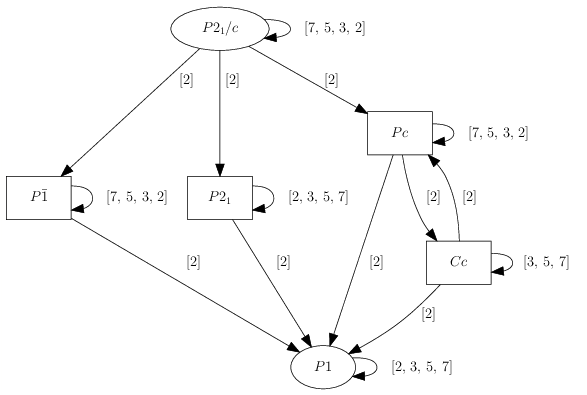
\includegraphics[width=0.5\linewidth]{figures/subgroupgraph.png}
    \caption{An example of a subgroup graph generated by the Bilbao Crystallographic Server web site program SUBGROUPGRAPH. It shows the subgroups of $P2_1/c$, which are $P\overline{1}$, $P 2_1$ and $P c$, which retain, respectively, the center of symmetry, the $2_1$ screw axis and the \textit{c}-glide. The subgroups of those space groups are shown as well.}
    \label{fig:subgroupgraph}
\end{figure}

\section{The BYU ISOTROPY Web Server}\label{ref:isotropy}
The Brigham Young University ISOTROPY Software Suite server, at web address \url{https://iso.byu.edu/}, is also an international treasure. It provides a collection of $\approx 20$ utility programs, which are largely motivated by representational analysis. Some of these offer very sophisticated analyses and graphical tools. The backbone of the site is the ISOTROPY program, which as far as I am aware is not in general distribution, but can be run online from the web site. Note that each utility entry has an extensive help page with documentation and, at least where I have looked, an annotated example. One of the really neat tools built into this website is a visualization program called IsoVIZ where one can vary the distortion modes generated by the programs and see how the structure is changed by the mode or combinations of modes. 

As noted before, if a CIF is generated on this web site that contains displacive, occupancy or magnetic distortion modes, when the CIF is read by GSAS-II, the distortion modes are converted to constraints that can then used in refinements. 
